\documentclass[conference]{IEEEtran}
\IEEEoverridecommandlockouts
% The preceding line is only needed to identify funding in the first footnote. If that is unneeded, please comment it out.
\usepackage{cite}
\usepackage{amsmath,amssymb,amsfonts}
\usepackage{algorithmic}
\usepackage{graphicx}
\usepackage{textcomp}
\usepackage{xcolor}
\def\BibTeX{{\rm B\kern-.05em{\sc i\kern-.025em b}\kern-.08em
    T\kern-.1667em\lower.7ex\hbox{E}\kern-.125emX}}
\begin{document}

\title{Understanding User Perspectives: Exploring Hoora Services, Product Development, and Sentiment Analysis\\
{\footnotesize \textsuperscript{}}
\thanks{}
}

\author{\IEEEauthorblockN{First Author }
\IEEEauthorblockA{\textit{Name of Department} \\
\textit{College Name, Location}\\
Email ID}
\and
\IEEEauthorblockN{Prof. Komal Kumbhare}
\IEEEauthorblockA{\textit{Name of Department} \\
\textit{College Name, Location}\\
komal.kumbhare@raisoni.net}
\and
\IEEEauthorblockN{First Author}
\IEEEauthorblockA{\textit{Name of Department} \\
\textit{College Name, Location}\\
Email ID}
\and
\IEEEauthorblockN{First Author}
\IEEEauthorblockA{\textit{Name of Department} \\
\textit{College Name, Location}\\
Email ID}
}

\maketitle

\begin{abstract}
The automotive industry's dynamic landscape is increasingly shaped by customer satisfaction, preferences, and the quality of auto care services. This research endeavours to unravel the intricacies of customer experiences through one-to-one calls and sentiment analysis. A comprehensive dataset, encompassing diverse demographic variables and detailed ownership attributes, was analysed to discern patterns and insights. Our findings reveal multifaceted aspects of automotive ownership, customer expectations, and the role of auto care services. Demographic information, such as gender, occupation, and vehicle details, has been meticulously examined. Moreover, sentiment analysis was employed to gauge customer sentiment regarding their vehicles, auto care, and service providers. The study unveils distinctive clusters of car owners based on their attitudes and expectations. We also scrutinise the factors that drive vehicle expenses and influence budgeting decisions. \\
The implications of our research are far-reaching, shedding light on the evolving landscape of automotive ownership and customer satisfaction. We discuss how auto care services can better align with the preferences and expectations of car owners. This study contributes to the broader understanding of customer-centric approaches within the automotive industry and lays the foundation for further research in this domain. 

\end{abstract}

\begin{IEEEkeywords}
Machine Learning Algorithms, Customer Satisfaction, Automotive Industry Auto Care Services, Enhancement Strategies 
\end{IEEEkeywords}

\section{Introduction}
This study delves into the intricate aspects of customer satisfaction, preferences, and the quality of auto care services within the automotive industry. It employs a robust dataset incorporating demographic variables and ownership attributes to conduct a thorough analysis of demographic patterns and sentiments. By identifying distinct clusters of car owners based on their attitudes and expectations, the research unveils insights into the diverse landscape of automotive ownership. 

Moreover, the research delves deeper than a cursory examination by investigating the variables that substantially affect automobile costs and shape drivers' financial choices. Using machine learning, sentiment analysis, and descriptive and predictive analytics, the study applies statistical tests to rigorously determine the significance of its findings. Applying cluster analysis is essential for finding automobile owner groups with related issues, which makes meaningful consumer segmentation possible.
Ultimately, the research aspires to offer valuable insights for stakeholders within the automotive industry. By shedding light on the evolving landscape of automotive ownership and aligning auto care services with the nuanced preferences of car owners, the study aims to contribute to the development of customer-centric approaches that enhance overall satisfaction and drive positive changes within the industry. 
 
\section{LITERATURE SURVEY}
This research explores the emerging field of survey informatics, merging survey methodology with computer science and engineering expertise [9]. It investigates cross-domain collaborations to advance survey practices, research, and technological innovations. Utilizing digital data sources and mobile sensor data, it aims to passively collect user information for surveys, reducing respondent burden while enabling efficient data gathering. Additionally, it examines incorporating gamification elements from computer games to improve survey participation and completion rates.
The author [1] paper presents a comprehensive review of autonomous car technology, exploring autonomous vehicle design, applications, testing approaches, and verification methodologies. Highlighting key technical challenges including validation, trust establishment, software robustness, computational demands management, safety, reliability, privacy, and security concerns. Investigated areas include deep learning for environment perception, machine learning for testing/validation, frameworks for real-world evaluations, mapping solutions, perception algorithms, and system architectures.
This research [2] investigates factors affecting the duration of car servicing and maintenance processes in India, emphasizing efficient service delivery and mechanics' problem-solving capabilities. The methodology encompasses surveying small-scale automotive repair businesses to analyse workforce demographics and operational practices. Furthermore, it conducts a survey of car owners to understand their decision-making criteria when requiring emergency repairs. Findings aim to inform strategies for improving the automotive aftermarket service industry benefiting both mechanics and customers.
The Author [6] explores theoretical underpinnings and limitations in developing deep learning networks tailored for autonomous driving applications. It evaluates architectures such as Deep Neural Networks (DNNs), Convolutional Neural Networks (CNNs), and Recurrent Neural Networks (RNNs) in the context of image recognition for self-driving vehicles. A central objective is devising specialized deep-learning techniques to enable reliable visual perception for autonomous cars. Advancement of these technologies is critical for facilitating robust perception and decision-making capabilities essential for self-driving vehicles. 
\section{METHODOLOGY}
\subsection{Data Collection}\label{AA}
The primary objective of this study was to gain insights into customer experiences and preferences in the context of auto care services. Data was collected through one-to-one calls [18], during which a series of structured questions were asked to car owners to get their feedback. The questions were designed to uncover specific issues and challenges they encountered during auto care services. The audio responses obtained from these calls were transcribed and used as the basis for further analysis. 
\subsection{Data Set}
The data set content basic information Customer Profile and Vehicle Details such as, Name, Phone No. Gender, Occupation, Vehicle Make, Brand of car, Vehicle Model, Vehicle Age, Smartphone Usage, Home Delivery Preferences were questions like Which e-commerce app do you use for home deliveries? What Kind of Phone do you use, Car Usage and Replacement Decision, Monthly Car Expenses and Routine Expenditures, Car Cleaning Preferences and Maintenance Knowledge, Car Cleaning Preferences and Maintenance Knowledge, Auto Care Service Needs and Concerns. 
\begin{figure}[htbp]
\centering
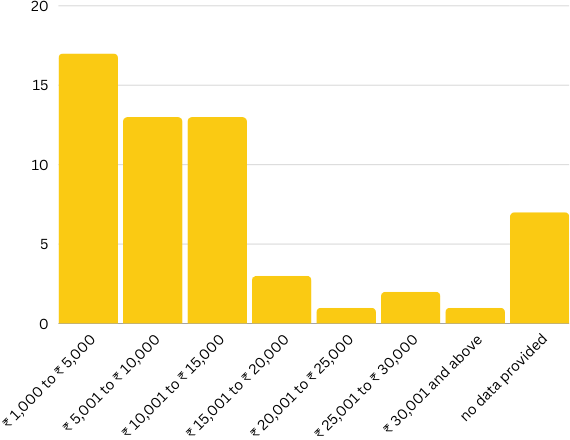
\includegraphics[scale=0.5]{Fig1.png}
\caption{How do you get your car cleaned?}
\label{fig}
\end{figure}
\subsection{Data Pre-processing}
The transcribed audio responses were subjected to preprocessing to ensure data quality and suitability for analysis.  This involved text cleaning, removal of any identifying information, and categorization of responses for specific questions. 
\subsection{Data Analysis}
To extract meaningful insights from the collected data, a Scombination of descriptive and predictive analytics was employed.
\subsection{Descriptive Analysis}
The transcribed responses were analysed to identify common themes and patterns in the issues faced by car owners during auto care services.  These findings were graphically represented to provide a visual summary of the most prevalent concerns. 
\subsection{Machine Learning Algorithms}
To further enhance the analysis, machine learning algorithms were utilised.  Random Forest, a supervised machine learning algorithm, logistic regression algorithm was employed to identify important features and factors contributing to customer dissatisfaction.  This allowed for the identification of key drivers behind customer concerns during auto care services [1]. 
\subsection{Sentiment Analysis}
A logistic regression algorithm was applied to assess the sentiment expressed in the responses. This sentiment analysis was instrumental in categorising responses as positive, negative, or neutral, providing a nuanced understanding of customer satisfaction and dissatisfaction. 
\subsection{Ethical Considerations}
It is crucial to note that all data collection and analysis procedures adhered to ethical standards, ensuring participant anonymity and data confidentiality. Informed consent was obtained from all participants, and personal information was redacted to protect their privacy. 
\begin{figure}[htbp]
\centering
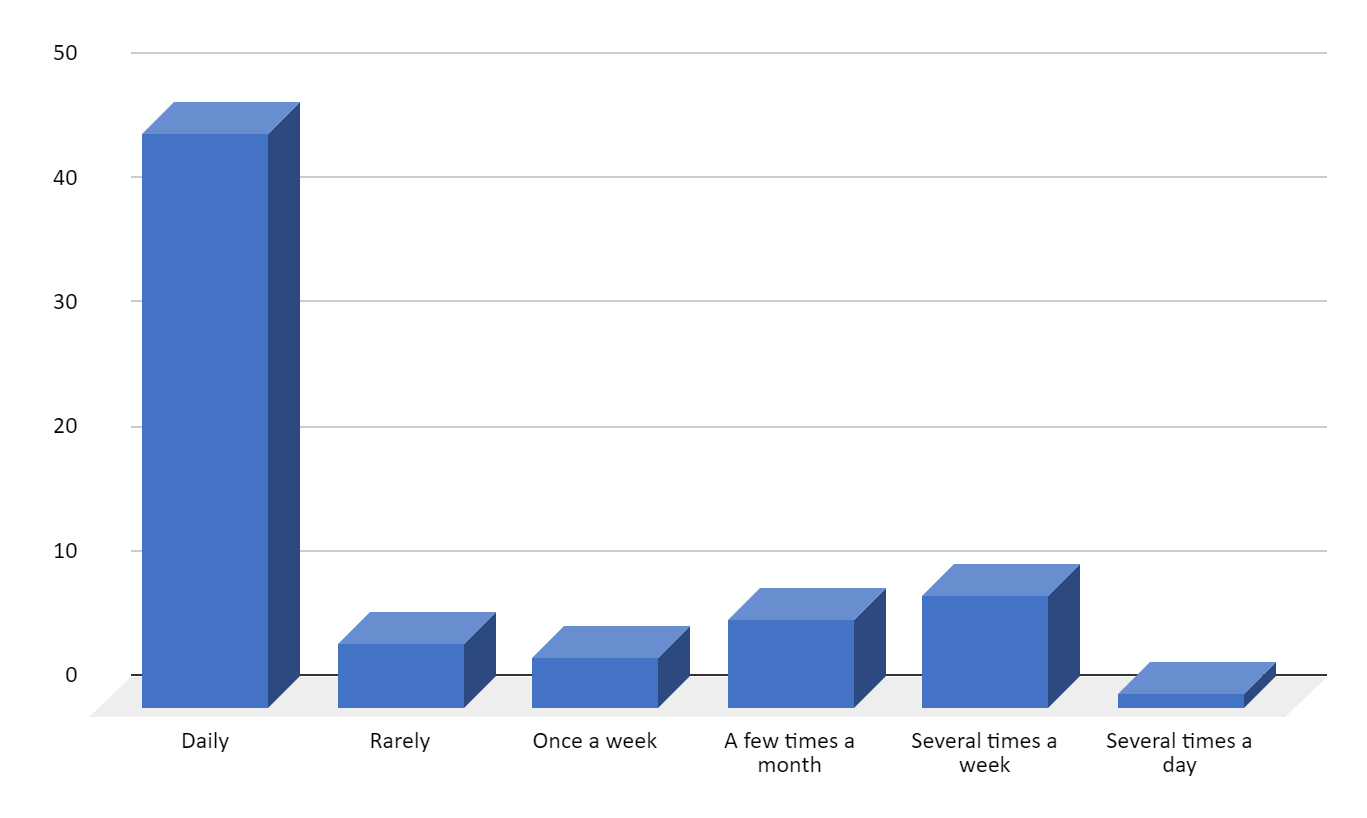
\includegraphics[scale=0.2]{Fig2.png}
\caption{Driving report}
\label{fig}
\end{figure}
\subsection{Statistical Analysis}
Statistical tests were conducted to establish the significance of the findings. This included chi-squared tests, t-tests, and regression analysis, where applicable, to assess the relationships between variables and customer satisfaction. 
\subsection{Cluster Analysis} 
Responses were subjected to cluster analysis [15] to identify distinct groups of car owners with similar concerns or preferences. This approach allowed for the segmentation [19] of the sample into meaningful customer segments based on their experiences and attitudes towards auto care services. 
\subsection{Algorithm used}
In addition to the justification for utilizing Random Forest in the research project, it's worth noting that the inclusion of Naive Bayes in the model adds a valuable dimension to the analytical approach. Naive Bayes is particularly well-suited for text classification tasks, making it an apt choice for sentiment analysis within the context of customer experiences in auto care services. 

The Naive Bayes algorithm operates on the principles of probability [16] and assumes independence between features, hence the "naive" designation. In the context of sentiment analysis, it can effectively handle textual data by considering the likelihood of a particular sentiment given the presence of certain words or phrases. This probabilistic nature allows for efficient and rapid classification of sentiments within a large dataset of customer reviews or feedback.
\begin{figure}[htbp]
\centering
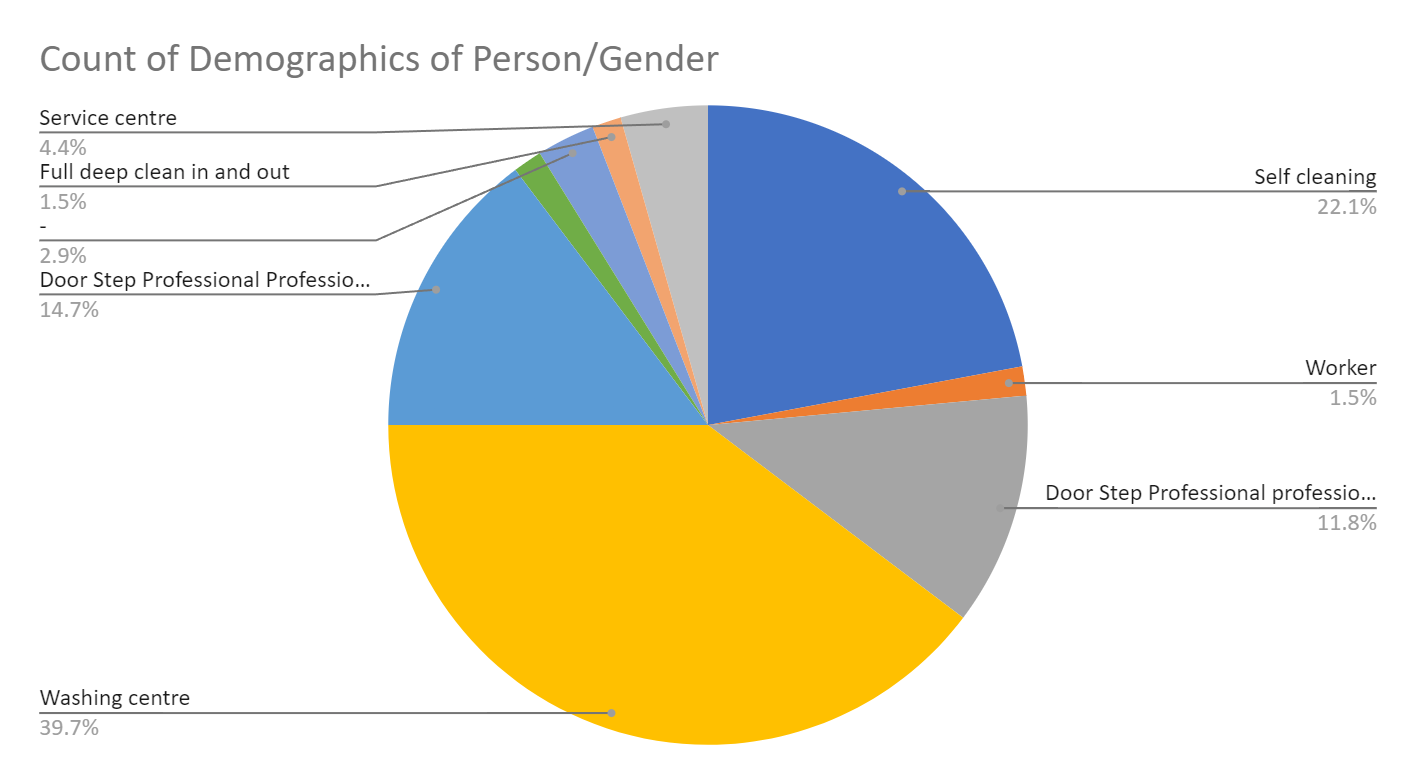
\includegraphics[scale=0.2]{Fig3.png}
\caption{Best way to clean car}
\label{fig}
\end{figure}
The integration of Naive Bayes alongside Random Forest creates a complementary synergy in the research model. While Random Forest excels in uncovering complex relationships and handling diverse data types, Naive Bayes enhances the model's proficiency in extracting sentiment-related insights from textual data. The combination of these two algorithms contributes to a more holistic analysis, ensuring that both structured and unstructured data are effectively leveraged to gain a nuanced understanding of the multifaceted landscape of customer experiences in auto care services. [4] 
\begin{figure}[htbp]
\centering
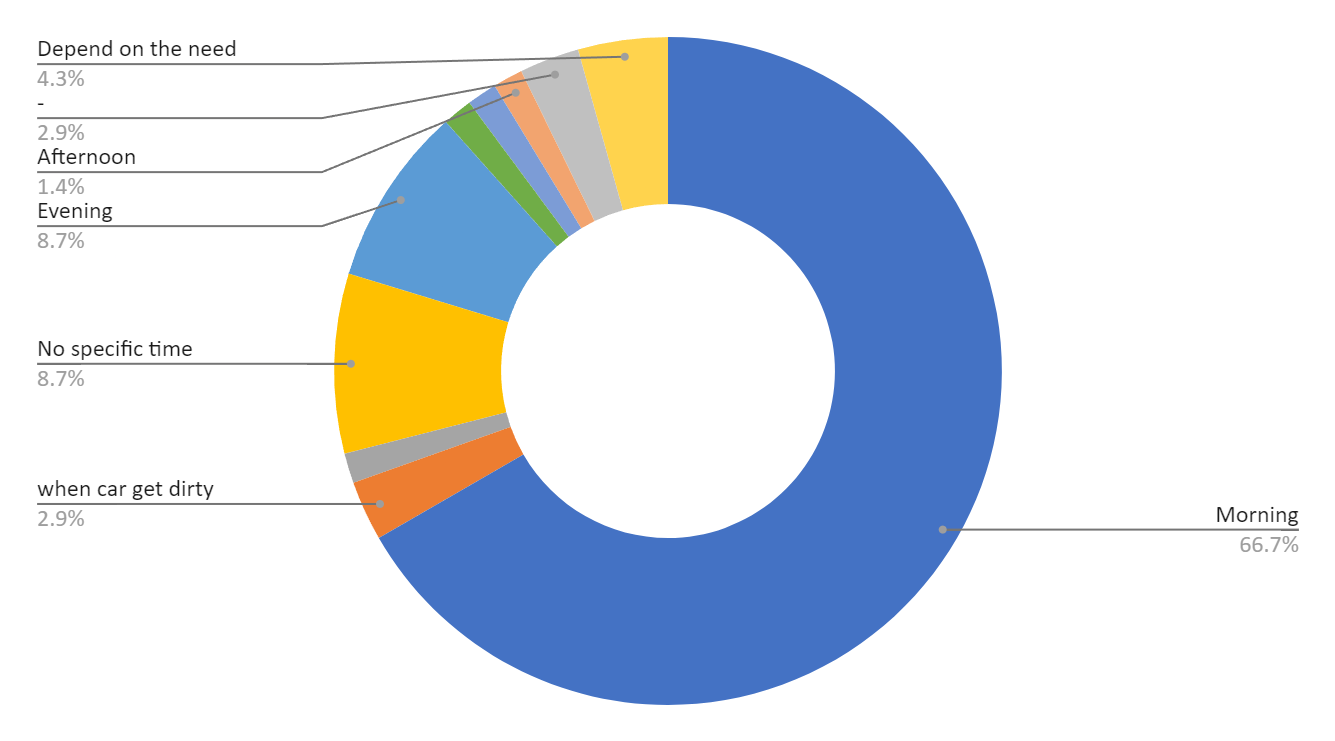
\includegraphics[scale=0.2]{Fig4.png}
\caption{Users prefer to clean their car}
\label{fig}
\end{figure}
\begin{itemize}
\item Random Forest: In machine learning, the Random [14] Forest ensemble learning technique is utilised for both classification and regression applications. During the training phase, it builds many decision trees and outputs the mode (for classification) or mean prediction (for regression) of each tree. 
\begin{equation}
    \hat{Y_{RF}} = \arg\max_k \left( \frac{1}{N} \sum_{i=1}^{N} \mathbb{I}(\hat{y_i}=k) \right)
\end{equation}

where:
\begin{itemize}
    \item $\hat{Y_{RF}}$ is the Random Forest prediction,
    \item $\hat{y_i}$ is the prediction of the $i$-th decision tree ,
    \item $I()$ is the indicator function. 
\end{itemize}
Random Forest Prediction (Regression): 
\begin{equation}
    \hat{Y_{RF}} =  \frac{1}{N} \sum_{i=1}^{N}\hat{y_i}
\end{equation}

\begin{figure}[htbp]
\centering
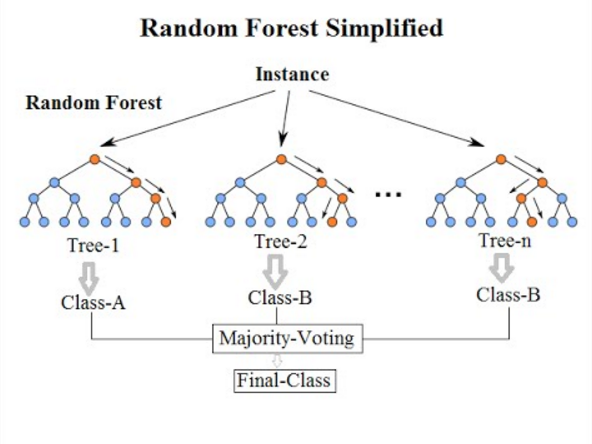
\includegraphics[scale=0.35]{Fig5.png}
\caption{Random forest graphical representation }
\label{fig}
\end{figure}

\item Naive Bayes: The Naive Bayes algorithm is a probabilistic classification method used in machine learning for text analysis and sentiment classification. It operates on the principles of probability, assuming independence between features. Naive Bayes is particularly effective in sentiment analysis, categorising textual data into predefined classes. It is suitable for large datasets and real-time applications, complementing ensemble learning techniques like Random Forest 
\begin{equation}
    \mathbb{P}(Class|Features)= \frac{ \mathbb{P}(Features|Class)\mathbb{P}(Class)}{\mathbb{P}(Features)}
\end{equation}
where:
\begin{itemize}
    \item $\mathbb{P}(Class|Features)$ is the posterior probability of the class given the observed features.
    \item $\mathbb{P}(Features|Class)$ is the likelihood of observing the features given the class. 
    \item $\mathbb{P}(Class)$ is the prior probability of the class. 
    \item $\mathbb{P}(Features)$ is the probability of observing the features. 
\end{itemize}
\end{itemize}
\subsection{Data Validation} 
To ensure the accuracy and reliability of the results, data validation and cross-validation techniques were employed. This included comparing the results obtained from different analytical methods and cross-referencing them with the original audio responses. 

The methodology presented here forms the foundation of the research process, enabling the extraction of valuable insights from the collected data. The combination of qualitative and quantitative approaches, including machine learning and sentiment analysis, allowed for a comprehensive understanding of customer experiences and preferences in the context of auto care services. [2] These methodological choices provide a robust basis for the subsequent discussion and interpretation of the research findings.  Obtained from different analytical methods and cross-referencing them with the original audio responses. 
The methodology presented here forms the foundation of the research process, enabling the extraction of valuable insights from the collected data. The combination of qualitative and quantitative approaches, including machine learning and sentiment analysis, allowed for a comprehensive understanding of customer experiences and preferences in the context of auto care services.  These methodological choices provide a robust basis for the subsequent discussion and interpretation of the research findings.

\section{RESULTS}
The results of our thorough analysis of a question-answering model's performance revealed serious shortcomings, with an accuracy rate of only 22% and an F1 score of 20%. These metrics highlight how difficult it is for the model to appropriately respond to requests. A thorough analysis of the model-specific factors has shown that the observed limitations can be attributed to the model's dependence on a simple recurrent neural network (RNN) architecture, possible limitations in the training dataset, and challenges in understanding complex question structures and contextual subtleties. To improve the model's performance, our study suggests a multimodal strategy.
To deal with complex linguistic structures, this approach involves data augmentation to add diversity and richness to the training dataset, investigating more advanced neural network architectures like transformer-based models and long short-term memory (LSTM) networks, integrating contextual information to improve understanding of query intent, and investigating the possibility of using ensemble learning techniques by combining models with different strengths. Our research suggests that the performance of the question-answering model can be significantly improved by addressing these identified limits and following the suggested improvements, guaranteeing its ability to provide consistent and correct answers for a greater variety of questions.

\begin{table}[htbp]
\caption{Model Accuracy}
\begin{center}
   
    \begin{tabular}{|c|c|}
        \hline
        Algorithm & Accuracy \\
        \hline
        Random Forest & 38 \% \\
        \hline
        Naive Bayes & 14 \% \\
        \hline
    \end{tabular}
    
    \end{center}
\end{table}

The models with the greatest accuracy scores Random Forest Regressor model were followed by the Naive Bayes.  

\section{CONCLUSION}
In the conclusion of the research study, we conducted an in-depth evaluation of a question-answering model's performance, revealing significant deficiencies with an accuracy rate of just 38% and an F1 score of 20%. These limitations were attributed to several factors, including the model's reliance on a basic recurrent neural network (RNN) architecture, issues with the training dataset, and challenges in interpreting complex question structures and context effectively.
To address these limitations and enhance the model's capabilities, we proposed a multi-faceted approach. This approach includes data augmentation techniques to introduce diversity and richness to the training dataset, exploring advanced neural network architectures such as long short-term memory (LSTM) networks and transformer-based models to handle complex linguistic structures, integrating contextual information to improve the model's comprehension of question intent, and considering ensemble learning techniques to combine models with distinct strengths.
These proposed enhancements hold the promise of substantially improving the model's performance, enabling it to provide reliable and accurate responses across a wider range of questions. By identifying limitations and providing actionable strategies to overcome them, this research contributes to the ongoing advancement of natural language processing and question-answering systems, paving the way for more sophisticated and effective AI-driven solutions in the future.
Continuous improvement strategies, such as gathering user feedback and extending sentiment analysis capabilities, will further enhance the app's features. Cross-platform integration will ensure a seamless experience across devices, while robust privacy measures will build user trust. This comprehensive approach aims to create a highly personalized, user-friendly, and valuable platform for auto care services. By implementing advanced technologies and a user-centric approach, Hoora seeks to position itself as a leader in the industry, providing exceptional value to users and maximizing customer satisfaction and loyalty.

\section{DISCUSSION}
The research paper employs a comprehensive methodology that combines qualitative and quantitative approaches, leveraging machine learning and sentiment analysis to enhance the understanding of customer-centric approaches within the automotive industry. Notably, the use of the Random Forest ensemble learning technique in classification and regression applications indicates a sophisticated analytical approach, allowing for robust insights. 
Sentiment analysis is a key component of the research, providing a deep understanding of consumer mindsets regarding their vehicles, auto care, and service providers. This qualitative aspect is complemented by descriptive analysis, which helps identify common themes and patterns in the issues faced by car owners during auto care services [6]. This combination of techniques ensures a holistic exploration of customer experiences. 
The paper's findings contribute to the evolving landscape of automotive ownership and customer satisfaction, emphasizing the importance of aligning auto care services with the preferences and expectations of car owners. The comprehensive understanding of customer experiences and preferences derived from the research provides actionable insights for stakeholders in the automotive industry. Ultimately, this research methodology lays the groundwork for informed decision-making, guiding stakeholders toward effective strategies that resonate with the dynamic needs of car owners in the realm of auto care services. 

\section{FUTURE SCOPE}
Future opportunities for Hoora include the integration of a personalized recommendation system and the use of customer traffic analysis for user interface optimization, with the goal of improving the user experience and maximizing customer retention. The personalized recommendation system uses users' past behaviour, car type preferences, demographics, and interactions to provide personalized car service recommendations and predict future costs. By dynamically adapting to user preferences over time, the system ensures relevance and usefulness. At the same time, turnover analysis provides an overview of user behaviour patterns and factors influencing attrition. This data helps optimize the user interface with a focus on improving engagement, satisfaction, and retention. Through user-cantered design, A/B testing, and iterative improvements based on traffic data, Hoora improves the app's usability and appeal.

Continuous improvement strategies, such as collecting user feedback and expanding sentiment analysis capabilities, further improves the functions of the program. . . Cross-board integration ensures a seamless user experience across all devices, while strong privacy measures increase user confidence. This comprehensive approach aims to create a highly personalized, user-friendly, and valuable platform for car care services. By adopting advanced technologies and a user-centric approach, Hoora aims to position itself as an industry leader, providing exceptional added value to users and maximizing customer satisfaction and loyalty.



\begin{thebibliography}{00}
\bibitem{b1} R. Hussain and S. Zeadally, "Autonomous Cars: Research Results, Issues, and Future Challenges," in IEEE Communications Surveys \& Tutorials, vol. 21, no. 2, pp. 1275-1313, Secondquarter 2019, doi: 10.1109/COMST.2018.2869360.
\bibitem{b2} A. Jain and S. Subhedar, "Reduction of servicing and maintenance time of car — A future need," 2016 International Conference on Advances in Human Machine Interaction (HMI), Kodigehalli, India, 2016, pp. 1-6, doi: 10.1109/HMI.2016.7449161. 
\bibitem{b3} Sumit Koul and Trissa Merrin Philip, "Customer Segmentation Techniques on E-Commerce", 2021
\bibitem{b4} I. Radoš, M. Hajnić and I. Radoš, "Digital transformation of monitoring customer behaviour in the cars sales," 2020 43rd International Convention on Information, Communication and Electronic Technology (MIPRO), Opatija, Croatia, 2020, pp. 1441-1445. 
\bibitem{b5} Y. -H. Lee, C. -C. Liang and K. -H. Chen, "The Influences of Sensory Effects on Car Interior Designs," 2019 IEEE Eurasia Conference on IOT, Communication and Engineering (ECICE), Yunlin, Taiwan, 2019, pp. 47-50
\bibitem{b6} J. Liu, "Survey of the Image Recognition Based on Deep Learning Network for Autonomous Driving Car," 2020 5th International Conference on Information Science, Computer Technology and Transportation (ISCTT), Shenyang, China, 2020, pp. 1-6,
\bibitem{b7} S. Khan, "The Improvised Three Wheeler Diesel Engine Vehicles of Bangladesh: Preliminary Survey," 2022 25th International Conference on Computer and Information Technology (ICCIT), Cox's Bazar, Bangladesh, 2022, pp. 827-832,
\bibitem{b8} L. Mingsong, "Study on Traffic Accident Investigation and Site Survey Evidence Based on Motor Vehicle Insurance," 2016 Eighth International Conference on Measuring Technology and Mechatronics Automation (ICMTMA), Macau, China, 2016, 
\bibitem{b9} A. Eck, L. -K. Soh, K. Olson, A. L. McCutcheon, J. Smyth and R. F. Belli, "Understanding the Human Condition through Survey Informatics," in Computer, vol. 48, no. 11, pp. 110-114, Nov. 2015, doi: 10.1109/MC.2015.327.
\bibitem{b10} T. Crnovrsanin, S. D. Bartolomeo, C. Wilson and C. Dunne, "Indy Survey Tool: A Framework to Unearth Correlations in Survey Data," 2023 IEEE Visualization and Visual Analytics (VIS), Melbourne, Australia, 2023, pp. 146-150, doi: 10.1109/VIS54172.2023.00038. 
\bibitem{b11} T. Kanij, R. Merkel and J. Grundy, "Lessons learned from conducting industry surveys in software testing," 2013 1st International Workshop on Conducting Empirical Studies in Industry (CESI), San Francisco, CA, USA, 2013, pp. 63-66, doi: 10.1109/CESI.2013.6618474. 
\bibitem{b12}	S. Atkar, S. Raut, S. Ninawe, R. Agrawal, C. Dhule and N. Chavhan, "Performance Comparison of Gradient Boosting and Random Forest for the Classification of False News," 2023 International Conference on Research Methodologies in Knowledge Management, Artificial Intelligence and Telecommunication Engineering (RMKMATE), Chennai, India, 2023, pp. 1-5, doi: 10.1109/RMKMATE59243.2023.10369302. 
\bibitem{b13}	H. Bhimarapu, S. Bhelkar, N. Chavhan, C. Dhule and R. Agrawal, "Customer Segmentation Based on E-Commerce using K-Mean Clustering," 2023 International Conference on Recent Advances in Science and Engineering Technology (ICRASET), B G NAGARA, India, 2023, pp. 1-5, doi: 10.1109/ICRASET59632.2023.10419925. 
\bibitem{b14}	Rahul Agrawal, Kapil Jajulwar and Urvashi Agrawal, "A Design Approach for Performance Analysis of Infants Abnormality Using K Means Clustering", 5th International Conference on Trends in Electronics and Informatics ICOEI 2021, pp. 992-997, 3-5, June 2021, ISBN 978-1-6654- 1571-2/21.
\bibitem{b15}	S. N. Atkar, R. Agrawal, C. Dhule, N. C. Morris, P. Saraf and K. Kalbande, "Speech Emotion Recognition using Dialogue Emotion Decoder and CNN Classifier", 2023 2nd International Conference on Applied Artificial Intelligence and Computing (ICAAIC), pp. 94-99, 2023.
\bibitem{b16} A. A. Deshmukh, S. D. B. Sonar, R. V. Ingole, R. Agrawal, C. Dhule and N. C. Morris, "Satellite Image Segmentation for Forest Fire Risk Detection using Gaussian Mixture Models", 2023 2nd International Conference on Applied Artificial Intelligence and Computing (ICAAIC), pp. 806-811, 2023.
\bibitem{b17}	14. Aditi Mukte and Urvashi Agrawal Rahul Agrawal, "Smart Data Transfer for Data Monetization", IEEE International Conference on Computational Intelligence amp;amp; Computing Applications 2021, 26-27 Nov.2021.
\bibitem{b18} A. Kesarwani, S. S. Chauhan and A. R. Nair, "Fake News Detection on Social Media using K-Nearest Neighbor Classifier", 2020 International Conference on Advances in Computing and Communication Engineering (ICACCE), pp. 1-4, 2020.
\bibitem{b19} N. Khan, M. U. Akram, A. Shah and S. A. Khan, "Important attributes of customer satisfaction in telecom industry: A survey-based study," 2017 4th IEEE International Conference on Engineering Technologies and Applied Sciences (ICETAS), Salmabad, Bahrain, 2017, pp. 1-7, doi: 10.1109/ICETAS.2017.8277858. 
\bibitem{b20} N. C. Khandelwal, M. M. Wanjari and B. Vidhale, "Review Paper on Speech Emotion Recognition," 2023 2nd International Conference on Futuristic Technologies (INCOFT), Belagavi, Karnataka, India, 2023, pp. 1-4, doi: 10.1109/INCOFT60753.2023.10425384

\end{thebibliography}
\vspace{12pt}


\end{document}
